\section{Aquisição e Condicionamento de Sinais}

O projeto eletrônico do sistema de processamentos de sinais e monitoramento
consiste em quatro módulos de sistemas de captura e condicionamento para os
seguintes sinais: temperatura corporal e do ambiente, resistência galvânica da pele
(GSR), acontecimento de quedas do usuário da cadeira de rodas e eletrocardiograma.

Para o circuito de monitoramento de sinais de temperatura, foi utilizado um sensor
de medição linear de temperatura LM35, fabricado pela \textit{Texas Instruments}.
O sensor foi selecionado por sua variação linear de tensão de saída com a
variação de temperatura, além do seu baixo consumo e alta precisão de medidas
de temperatura com rápida resposta e sua faixa de captura de -55 à 150 graus Celsius,
tornando-o viável para monitoramento de temperaturas corporais e ambientais.
Tanto o circuito quanto o sistema embarcado foram projetados e dimensionados
para tratar de sua variação linear de 10 $mV$ em sua saída a cada 1 grau de variação
na temperatura\footnote{\url{http://www.ti.com/lit/ds/symlink/lm35.pdf}}.

Foram também realizados testes e algoritmos para medição da temperatura corporal com
termistores NTC, porém, os mesmo mostraram-se menos acurados devido ao seu comportamento
não linear dado pela equação de \textit{Equação de Steinhart-Hart}
\footnote{\url{lens.unifi.it/ew/dwl.php?dwl...mtyp=application/pdf}} e problemas de arredondamento
de valores capturados pelo sistema embarcado. Dessa forma, foi decidido o uso do sensor LM35.

O sensor fabricado para medição da temperatura corporal, apresentado na \ref{fig:temp_ele},
é aplicado à superfície da pele, no antebraço, possibilitando leitura facilitada
e de forma menos invasiva. Uma vez em contato com o corpo do usuário,
o sensor apresenta alteração nos valores lineares de temperatura até o momento de
estabilidade com a temperatura corporal.

\begin{figure}
    \begin{center}
        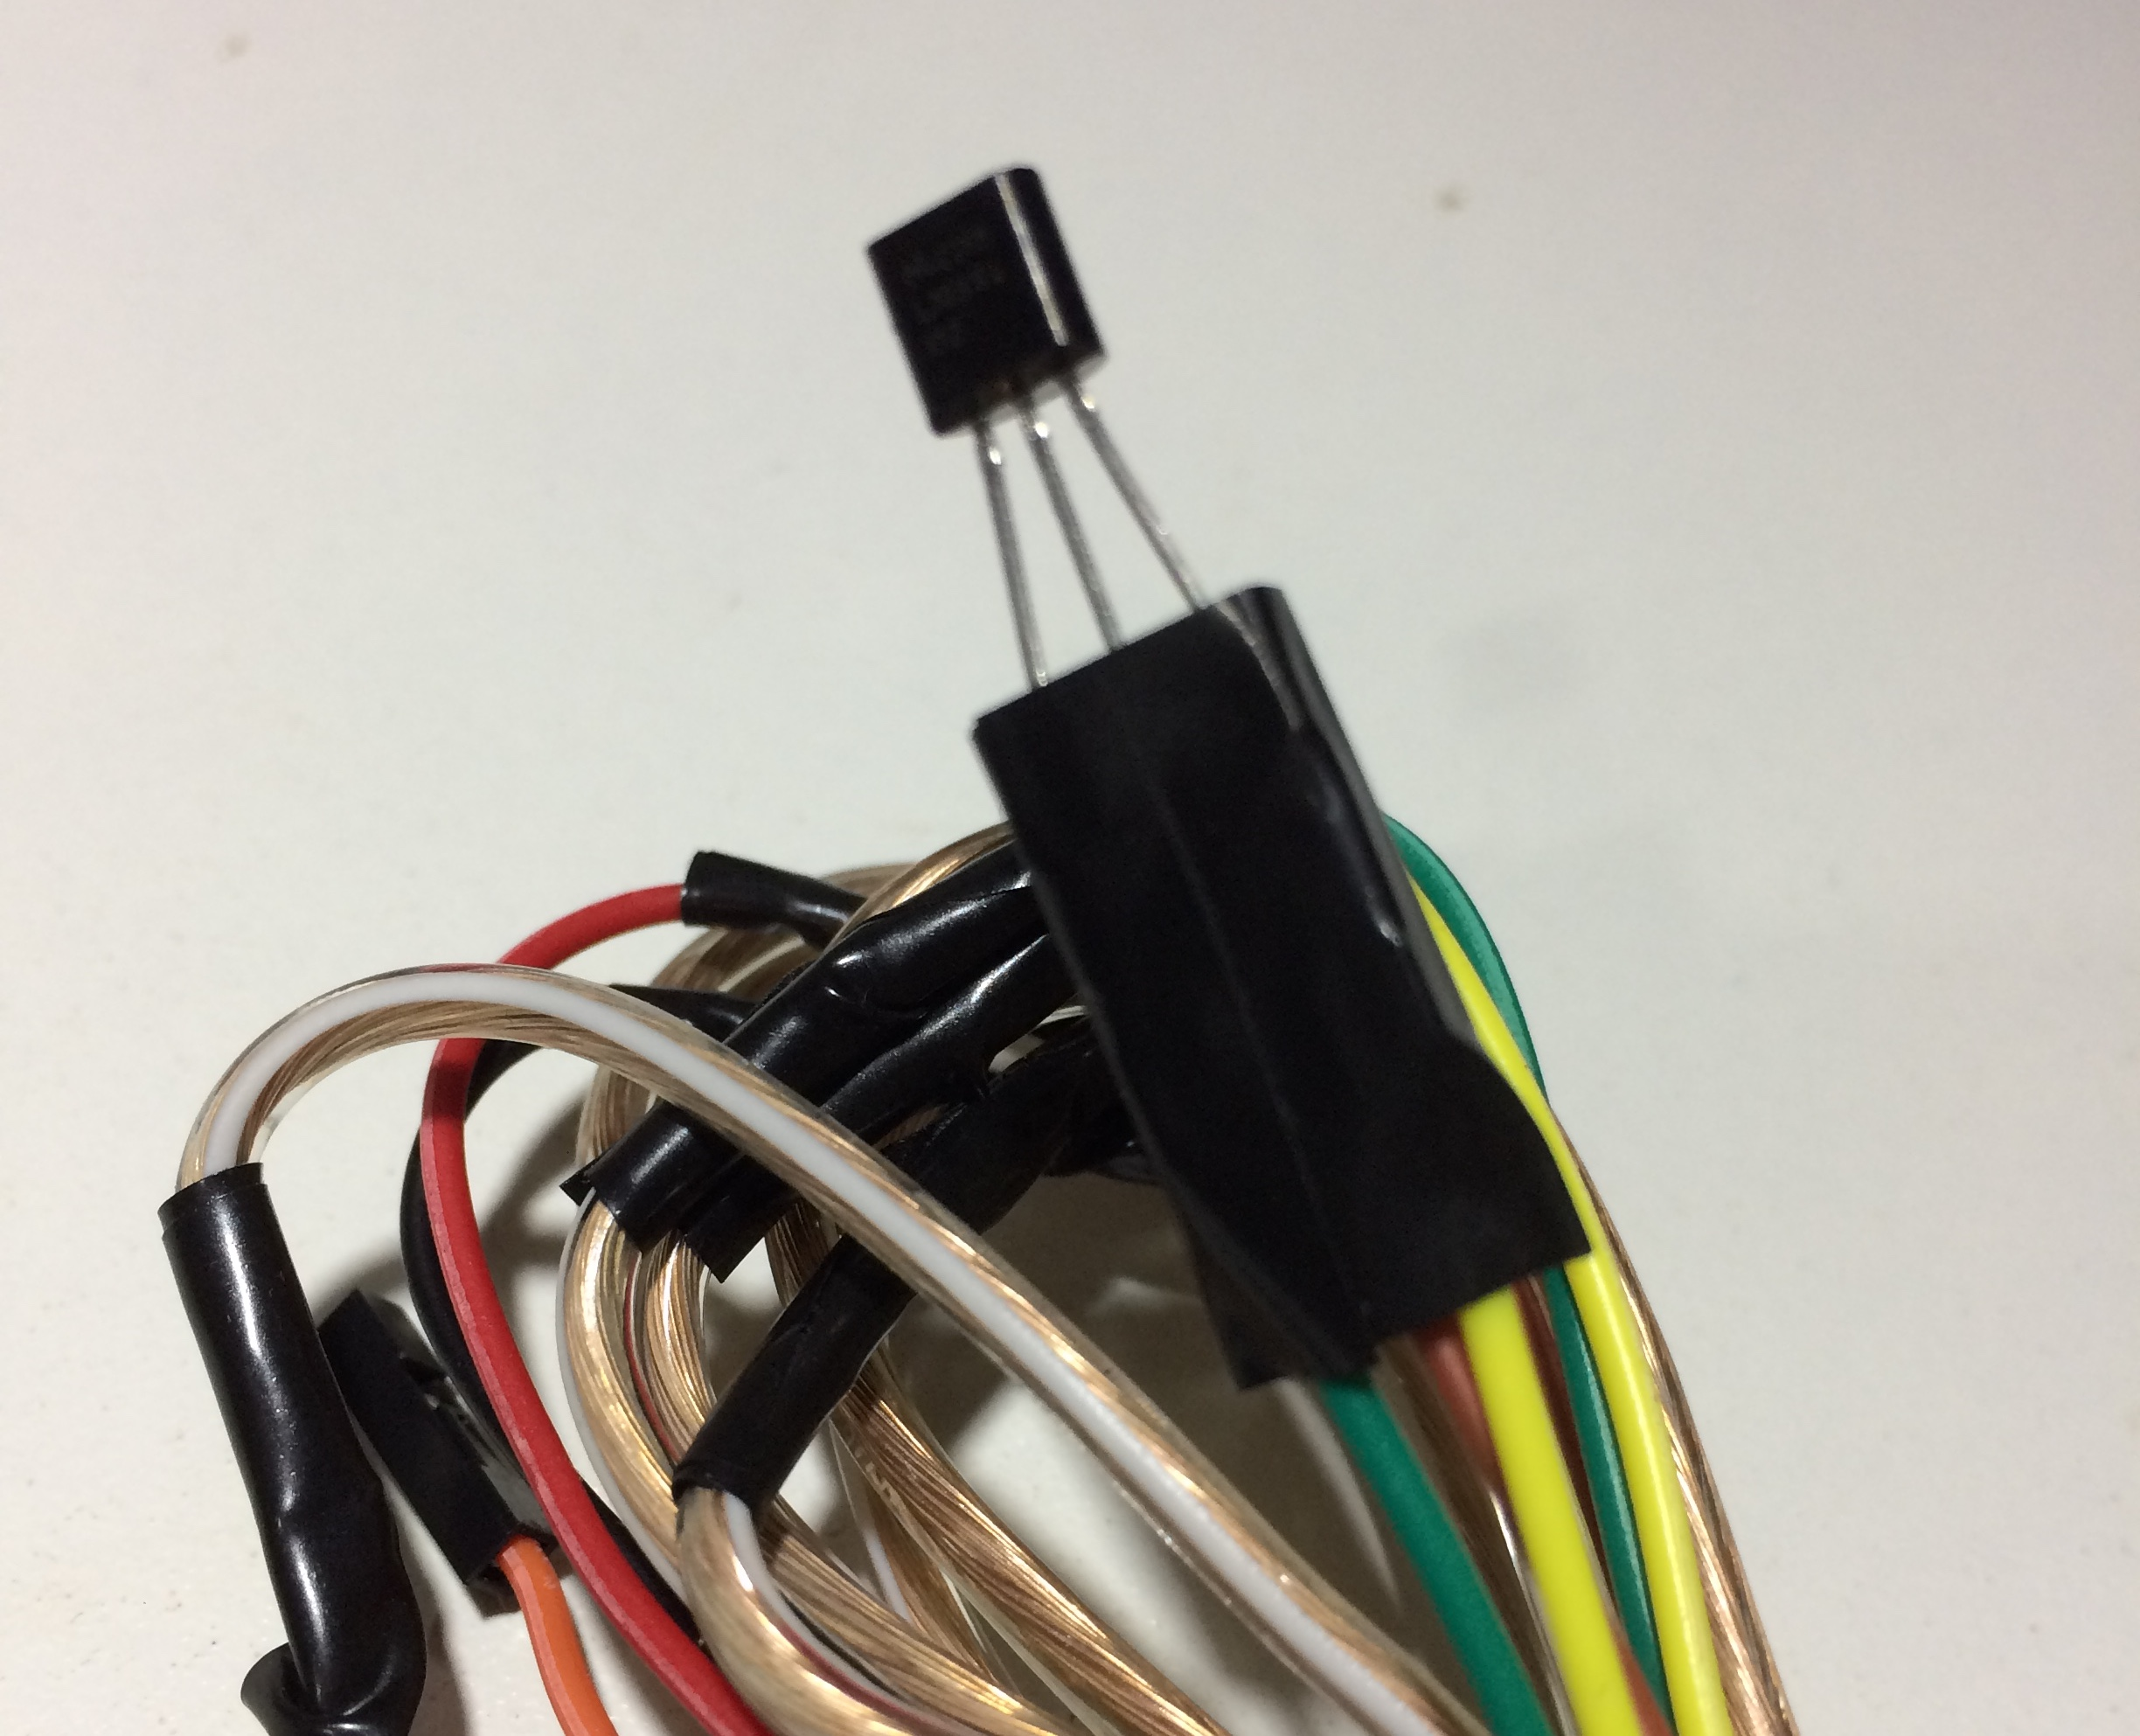
\includegraphics[scale=0.1]{figuras/temp_ele.jpg}
    \end{center}
    \caption{Sensor para medição de temperatura corporal.}
    \label{fig:temp_ele}
\end{figure}


O sistema de monitoramento de sinais de resistência galvânica da pele (GSR),
tem como principal função o monitoramento de variações na umidade da pele do
usuário, podendo indicar níveis perigosos de estresse ou até mesmo colapsos de
hipoglicemia ou por fraqueza por falta de alimentação. O sistema consiste em
dois eletrodos fabricados, como visto na na \ref{fig:gsr_ele}, para contato com o
antebraço do usuário, com uma distância fixa de 5 $cm$ entre eles, dessa forma,
mantendo os valores das medições confiáveis para cada usuário com diferentes tipos de pele.

\begin{figure}
    \begin{center}
        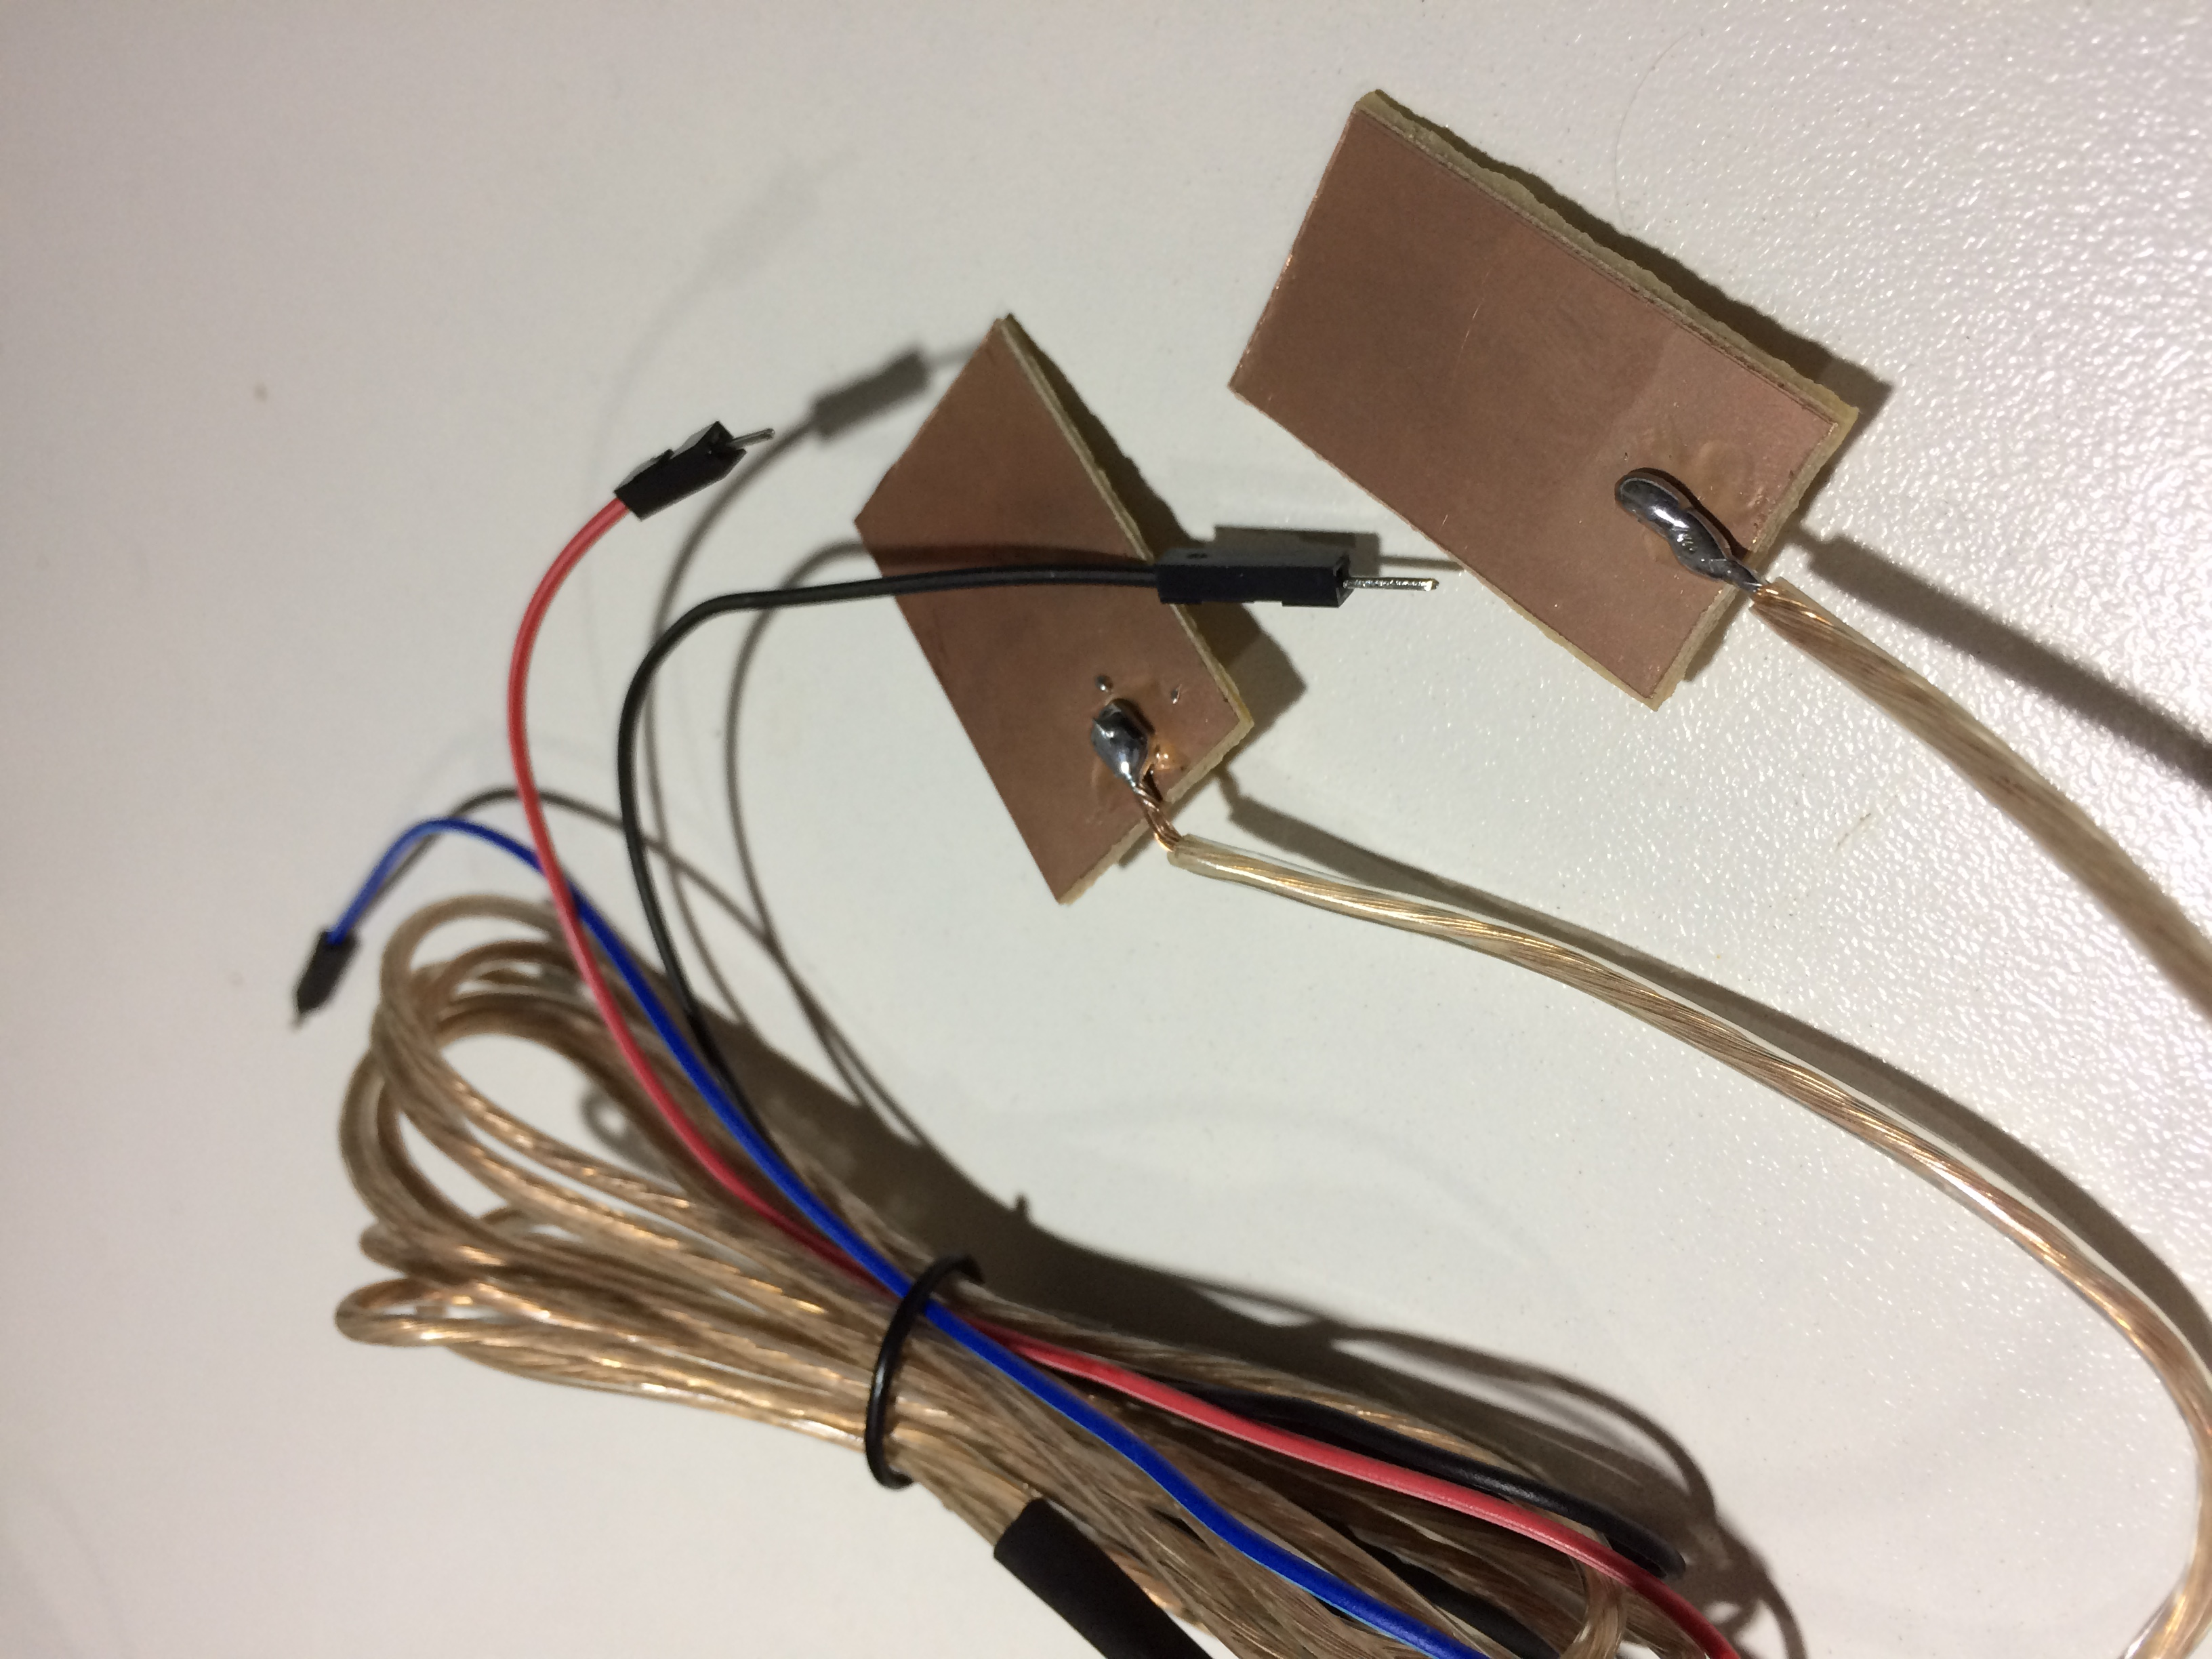
\includegraphics[scale=0.1]{figuras/gsr_ele.jpg}
    \end{center}
    \caption{Eletrodos fabricados para medição de umidade e resistência galvânica da pele.}
    \label{fig:gsr_ele}
\end{figure}

Além disso, o circuito, visto na Figura \ref{fig:gsr_circ} embarcado conta com um
capacitor de acoplamento para o contato com a pele
humana e um resistor de alta impedância para a medição da variação da resistência da pele
por divisor de tensão. O sistema foi simplificado para que pudesse ser implementado junto
aos cabos dos eletrodos, de forma a utilizar o mínimo de espaço possível na cadeira de rodas.

\begin{figure}
    \begin{center}
        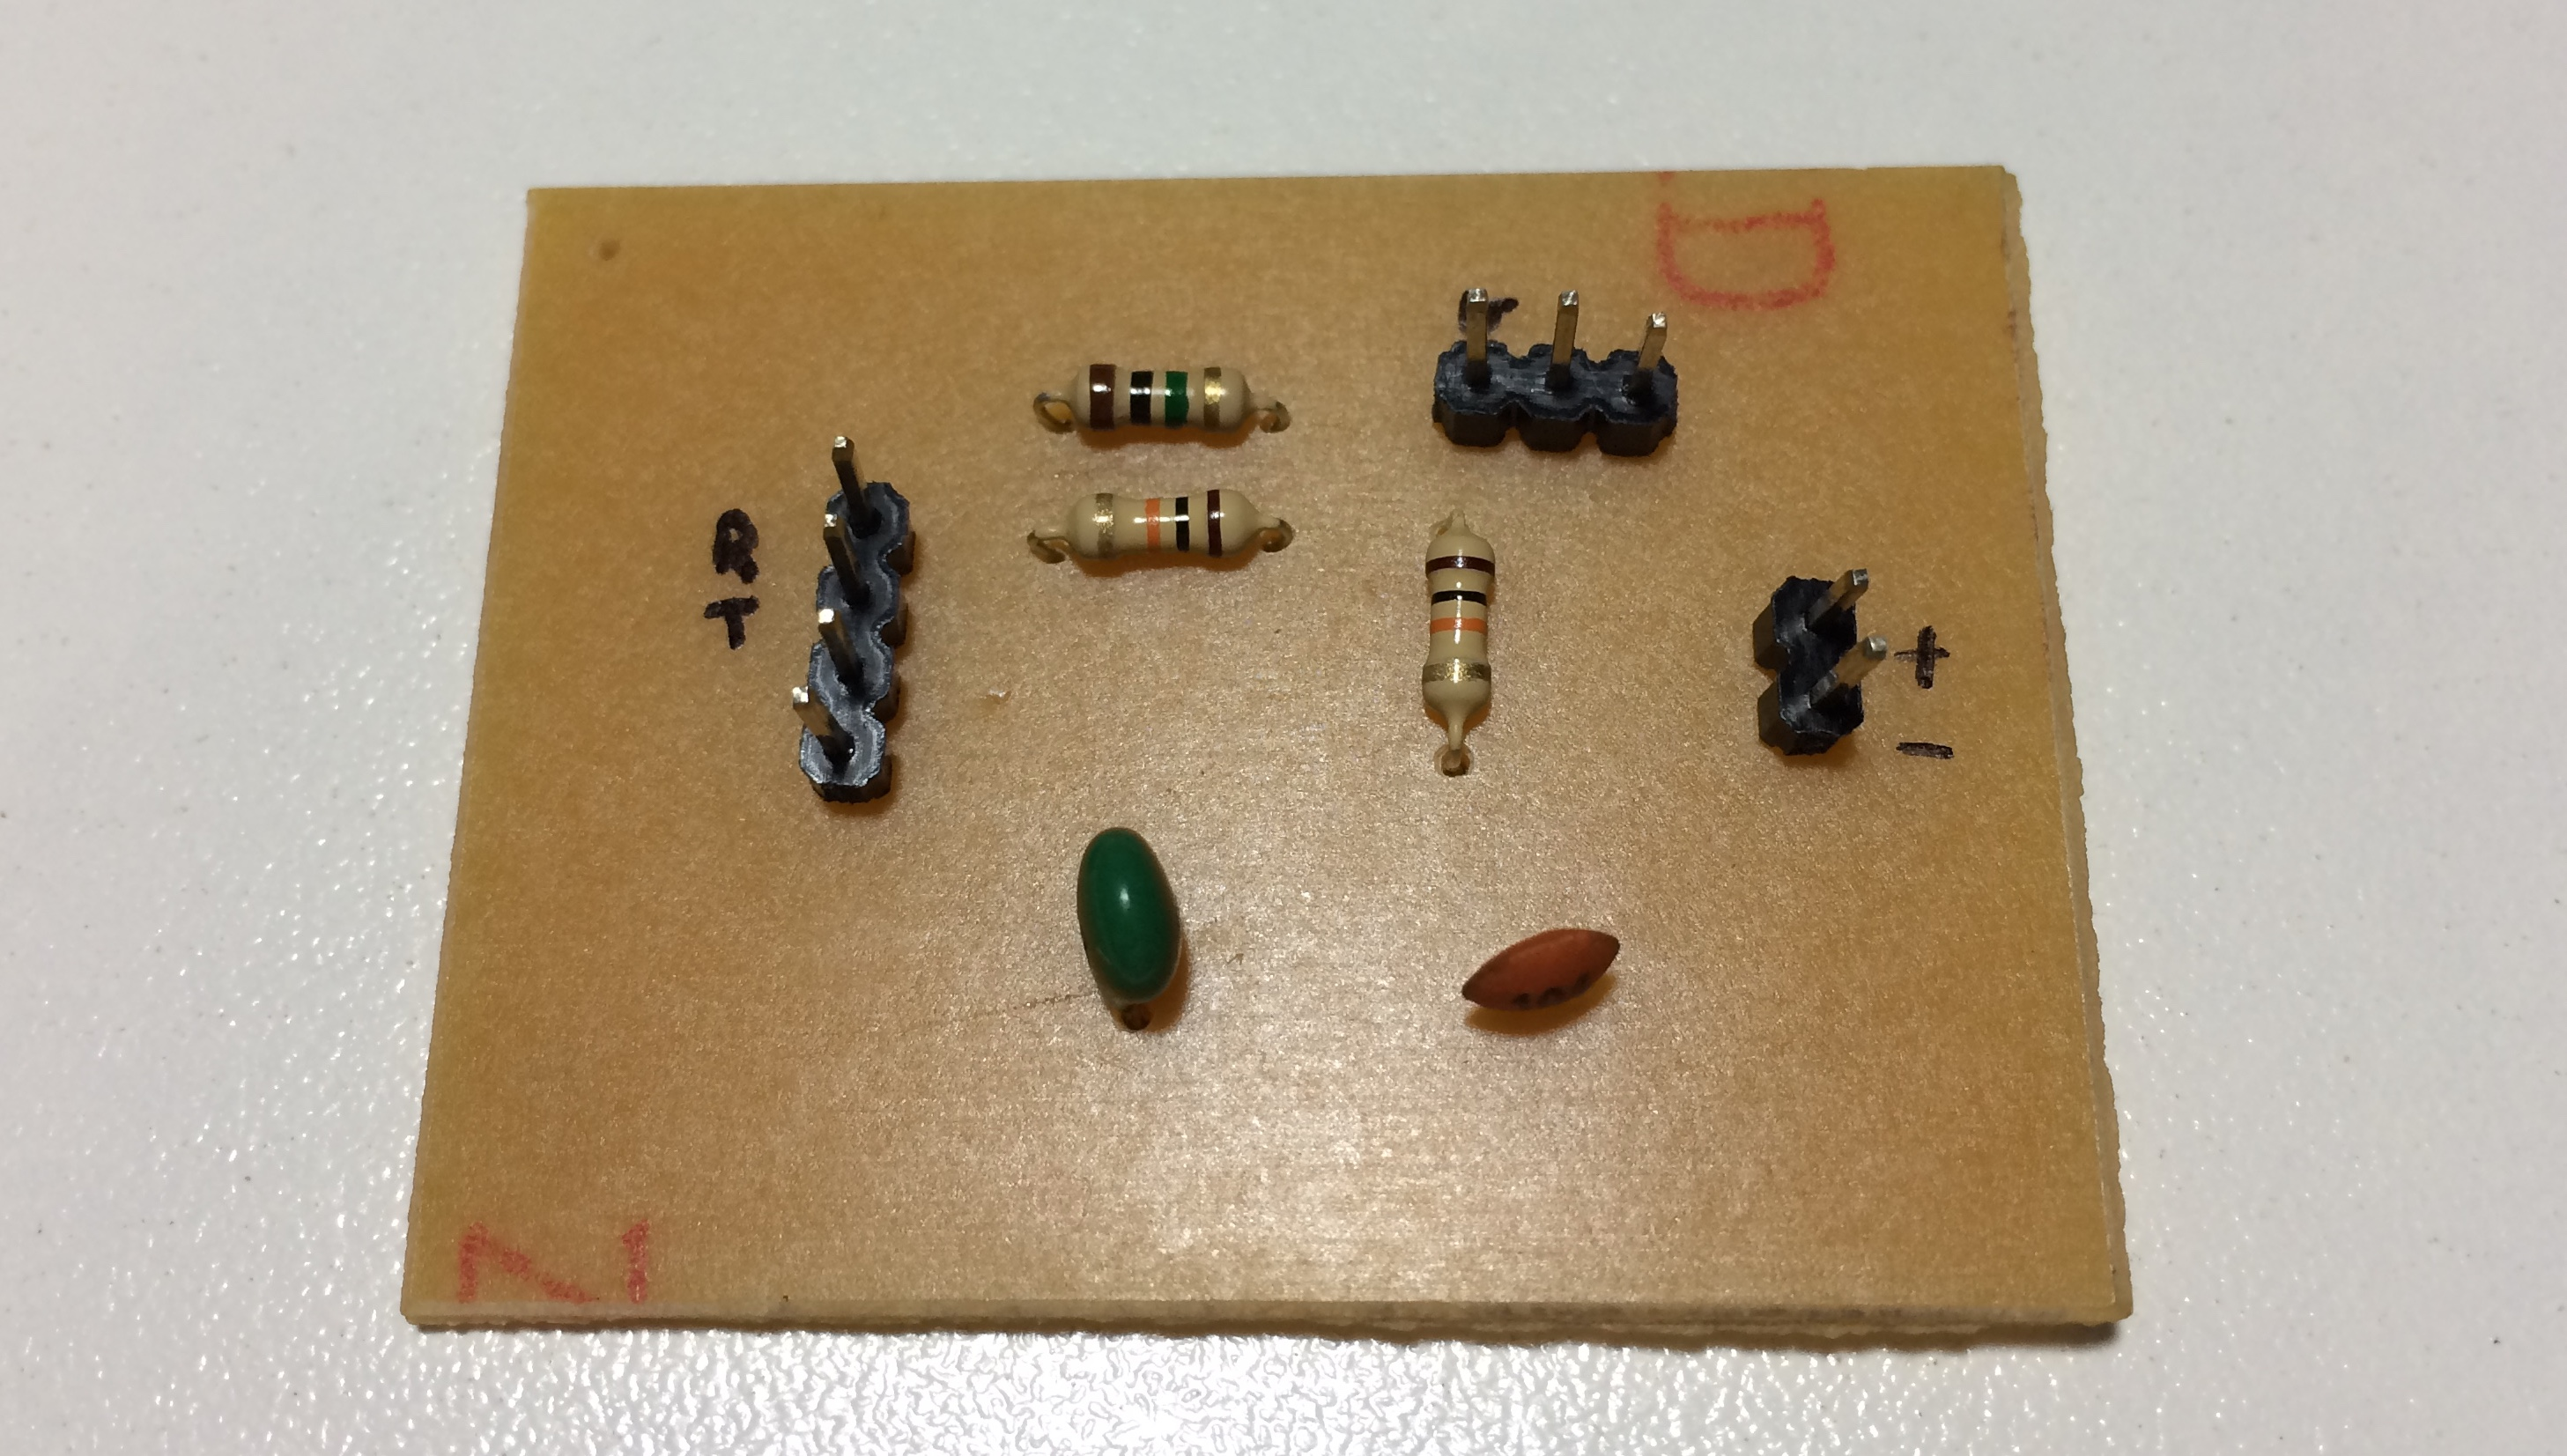
\includegraphics[scale=0.1]{figuras/gsr_circ.JPG}
    \end{center}
    \caption{Circuito para captura de umidade da pele por GSR.}
    \label{fig:gsr_circ}
\end{figure}

O algoritmo para o monitoramento da resistência galvânica e umidade conta com
comparadores para diferentes status do usuário, podendo alertar quando o usuário
não está realizando a medição, quando apresenta características normais para sua
pele ou quando o usuário encontra-se em situação de risco. O sistema embarcado para
o monitoramento e integração com o \textit{middleware} foi programado em linguagem Python.

O sistema de alerta de quedas é responsável por enviar alertas para o servidor
caso o usuário encontre-se fora da cadeira, indicando que o mesmo caiu da cadeira
e necessita de auxílio urgente. Para esse sistema, apresentado na Figura \ref{fig:fall_ele} foi desenvolvido um circuito
com um sistema de medição de distância e presença utilizando um módulo com sensor
piezoelétrico. O sistema é responsável pelo monitoramento de variações de tensão
no sensor, possibilitando o processamento dessa variação, alertando a presença
ou não do usuário na cadeira de rodas. O sensor piezoelétrico é inserido no assento
da cadeira para que o mesmo esteja pressionado durante todo o momento que o usuário
esteja sentado na cadeira, e dessa forma, o algoritmo é capaz de alertar caso a
presença do usuário na cadeira não seja identificada.

\begin{figure}
    \begin{center}
        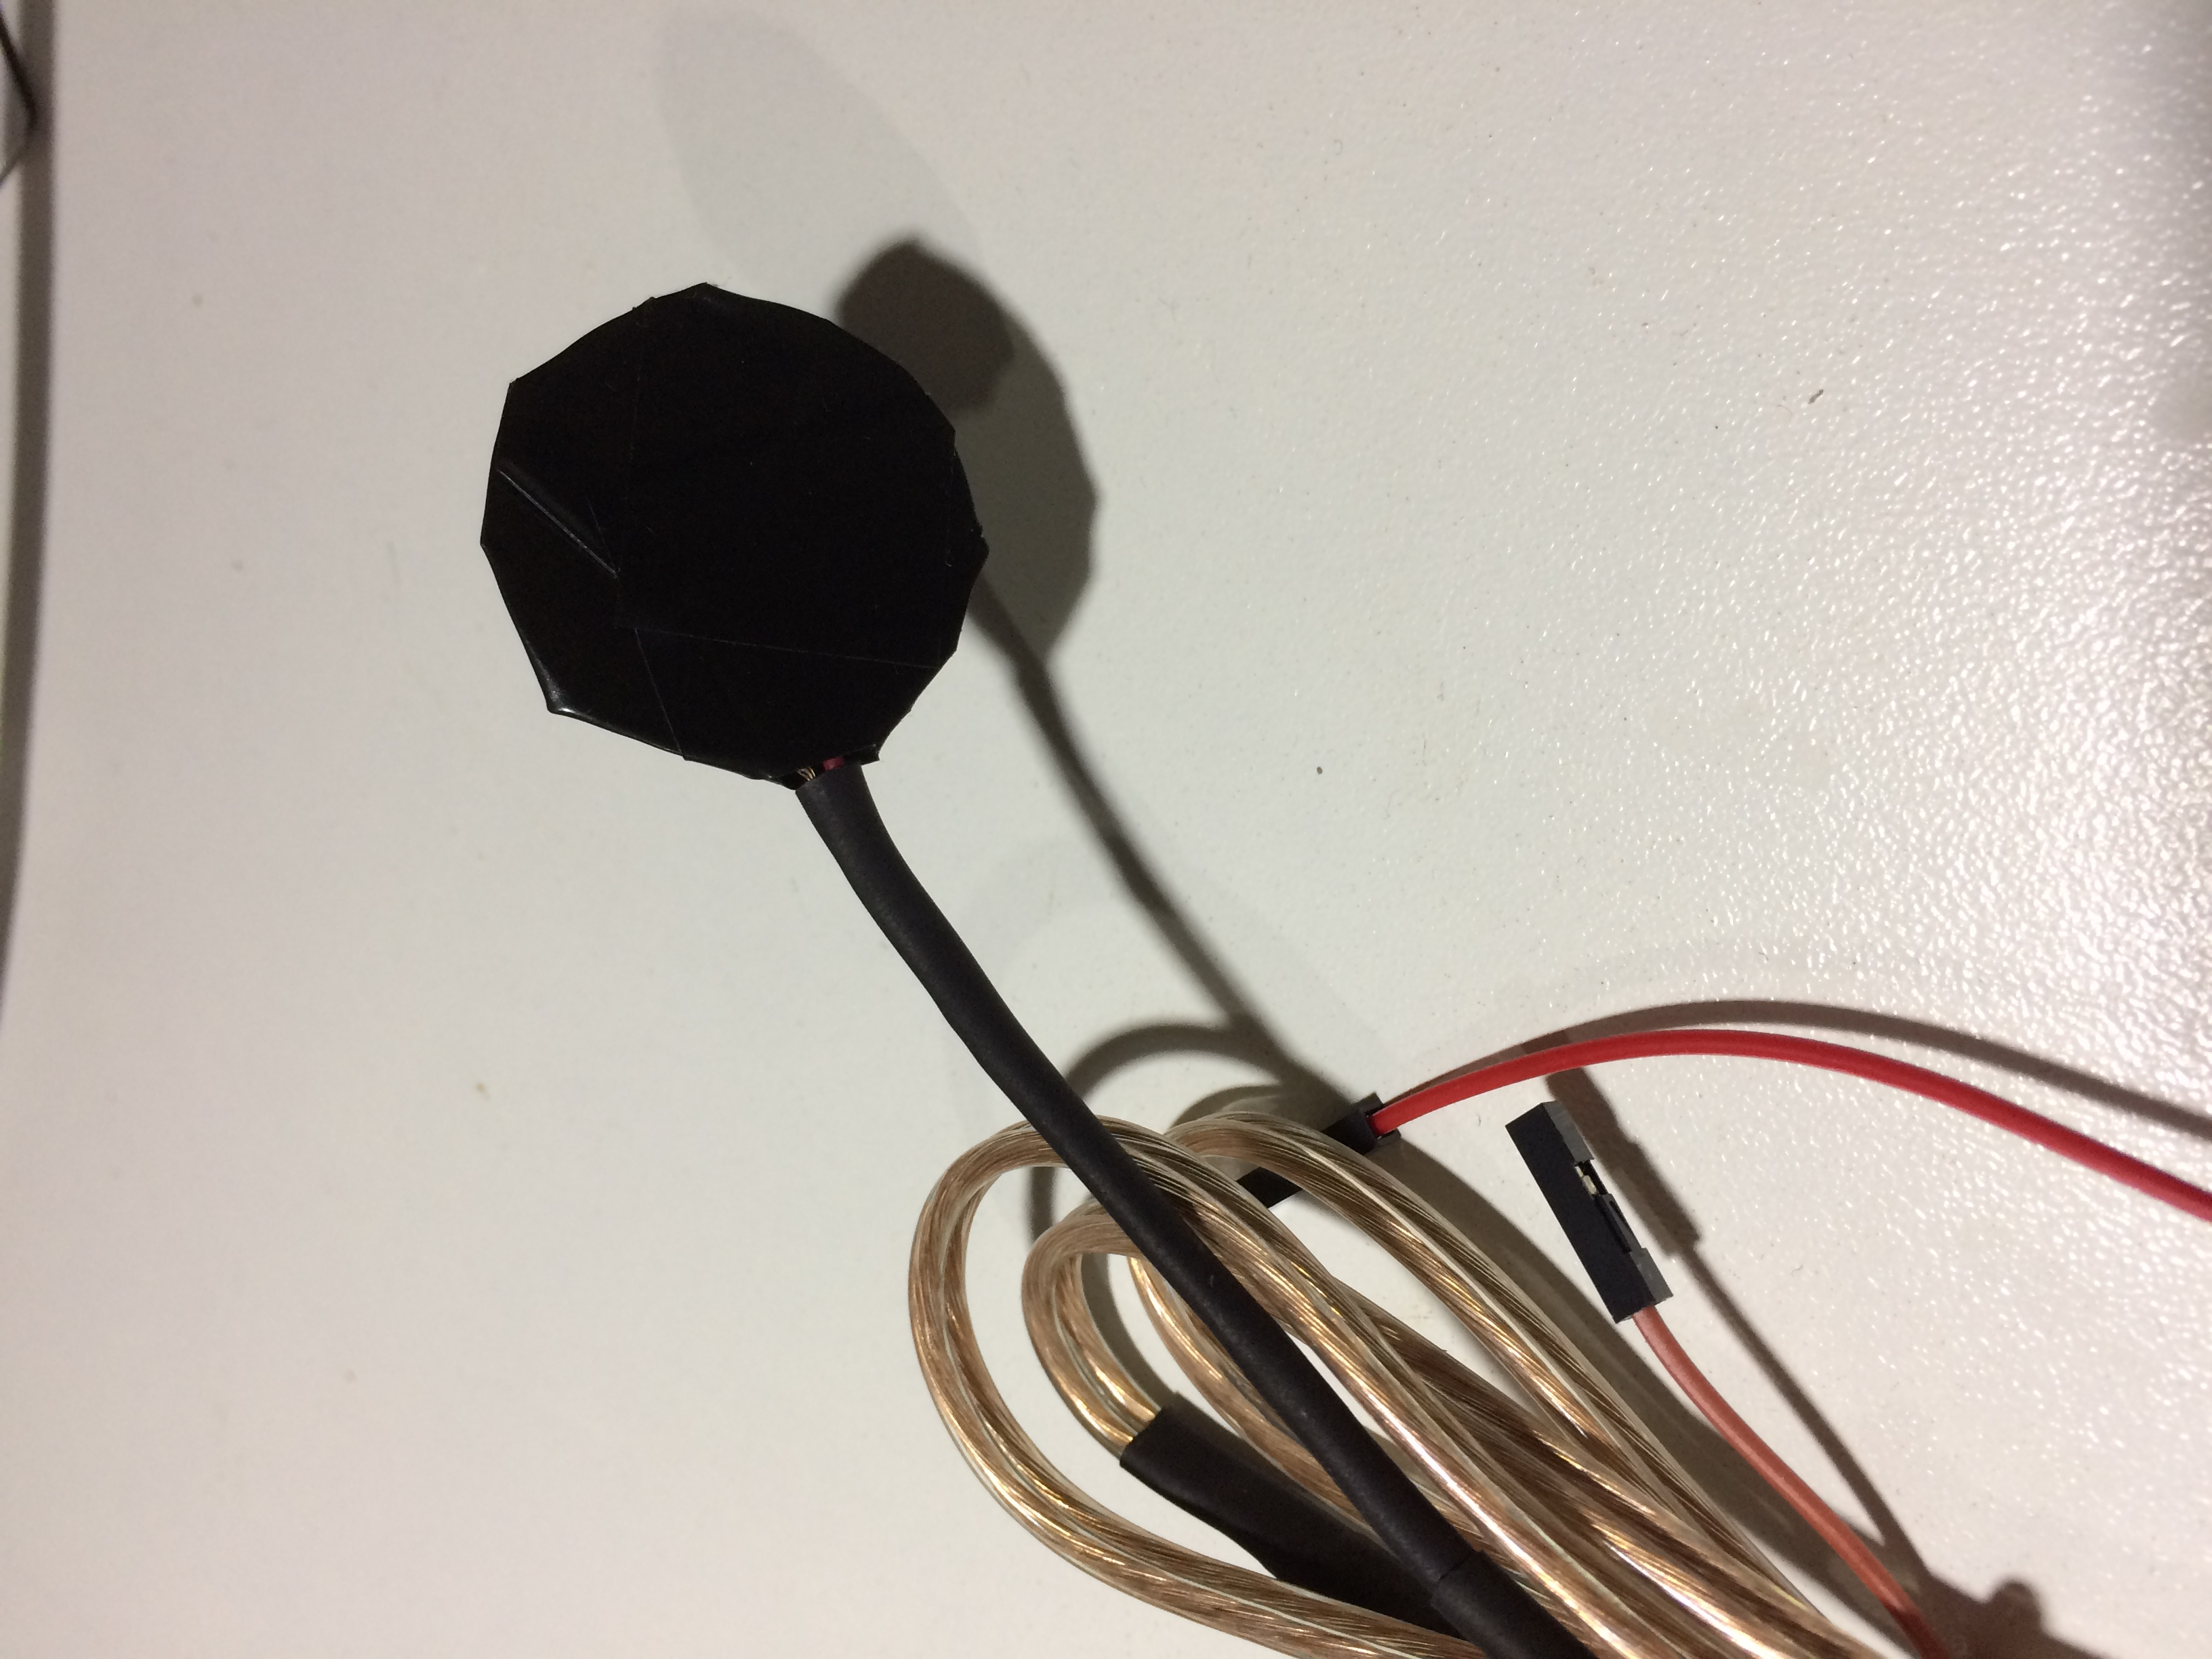
\includegraphics[scale=0.1]{figuras/fall_circ.png}
    \end{center}
    \caption{Sensor de presença do usuário na cadeira de rodas.}
    \label{fig:fall_ele}
\end{figure}

O sistema de monitoramento dos sinais de eletrocardiografia, apresentado na \ref{fig:ecg_circ}
foi desenvolvido para captura dos sinais de pulso cardíaco a partir de eletrodos
conectados ao antebraço do usuário, para que as medidas e a captura do sinais seja
feita da forma menos invasiva possível. Para isso, o circuito deve ser capaz de
capturar o sinal de ECG com precisão e assim, foi decidido pelo uso de um amplificador
de instrumentação INA 128p, fabricado pela \textit{Texas Instruments}\footnote{\url{http://www.ti.com/lit/ds/symlink/ina129.pdf}},
principalmente por suas características de alta rejeição de CMRR, além de ganho de fácil regulagem.
Além do amplificador de instrumentação, foram projetados filtros passa-baixa para
rejeição de frequências acima de 100Hz que possam interferir no sinal de eletrocardiograma,
que para monitoramento, variam entre baixas frequências de 0.5Hz e 40Hz\footnote{ Yazıcıoglu RF, van Hoof C,
Puers R. Biopotential Readout Circuits for Portable Acquisition Systems, 2009,
Springer Science, ISBN: 978-1-4020-9092-9)}.

\begin{figure}
    \begin{center}
        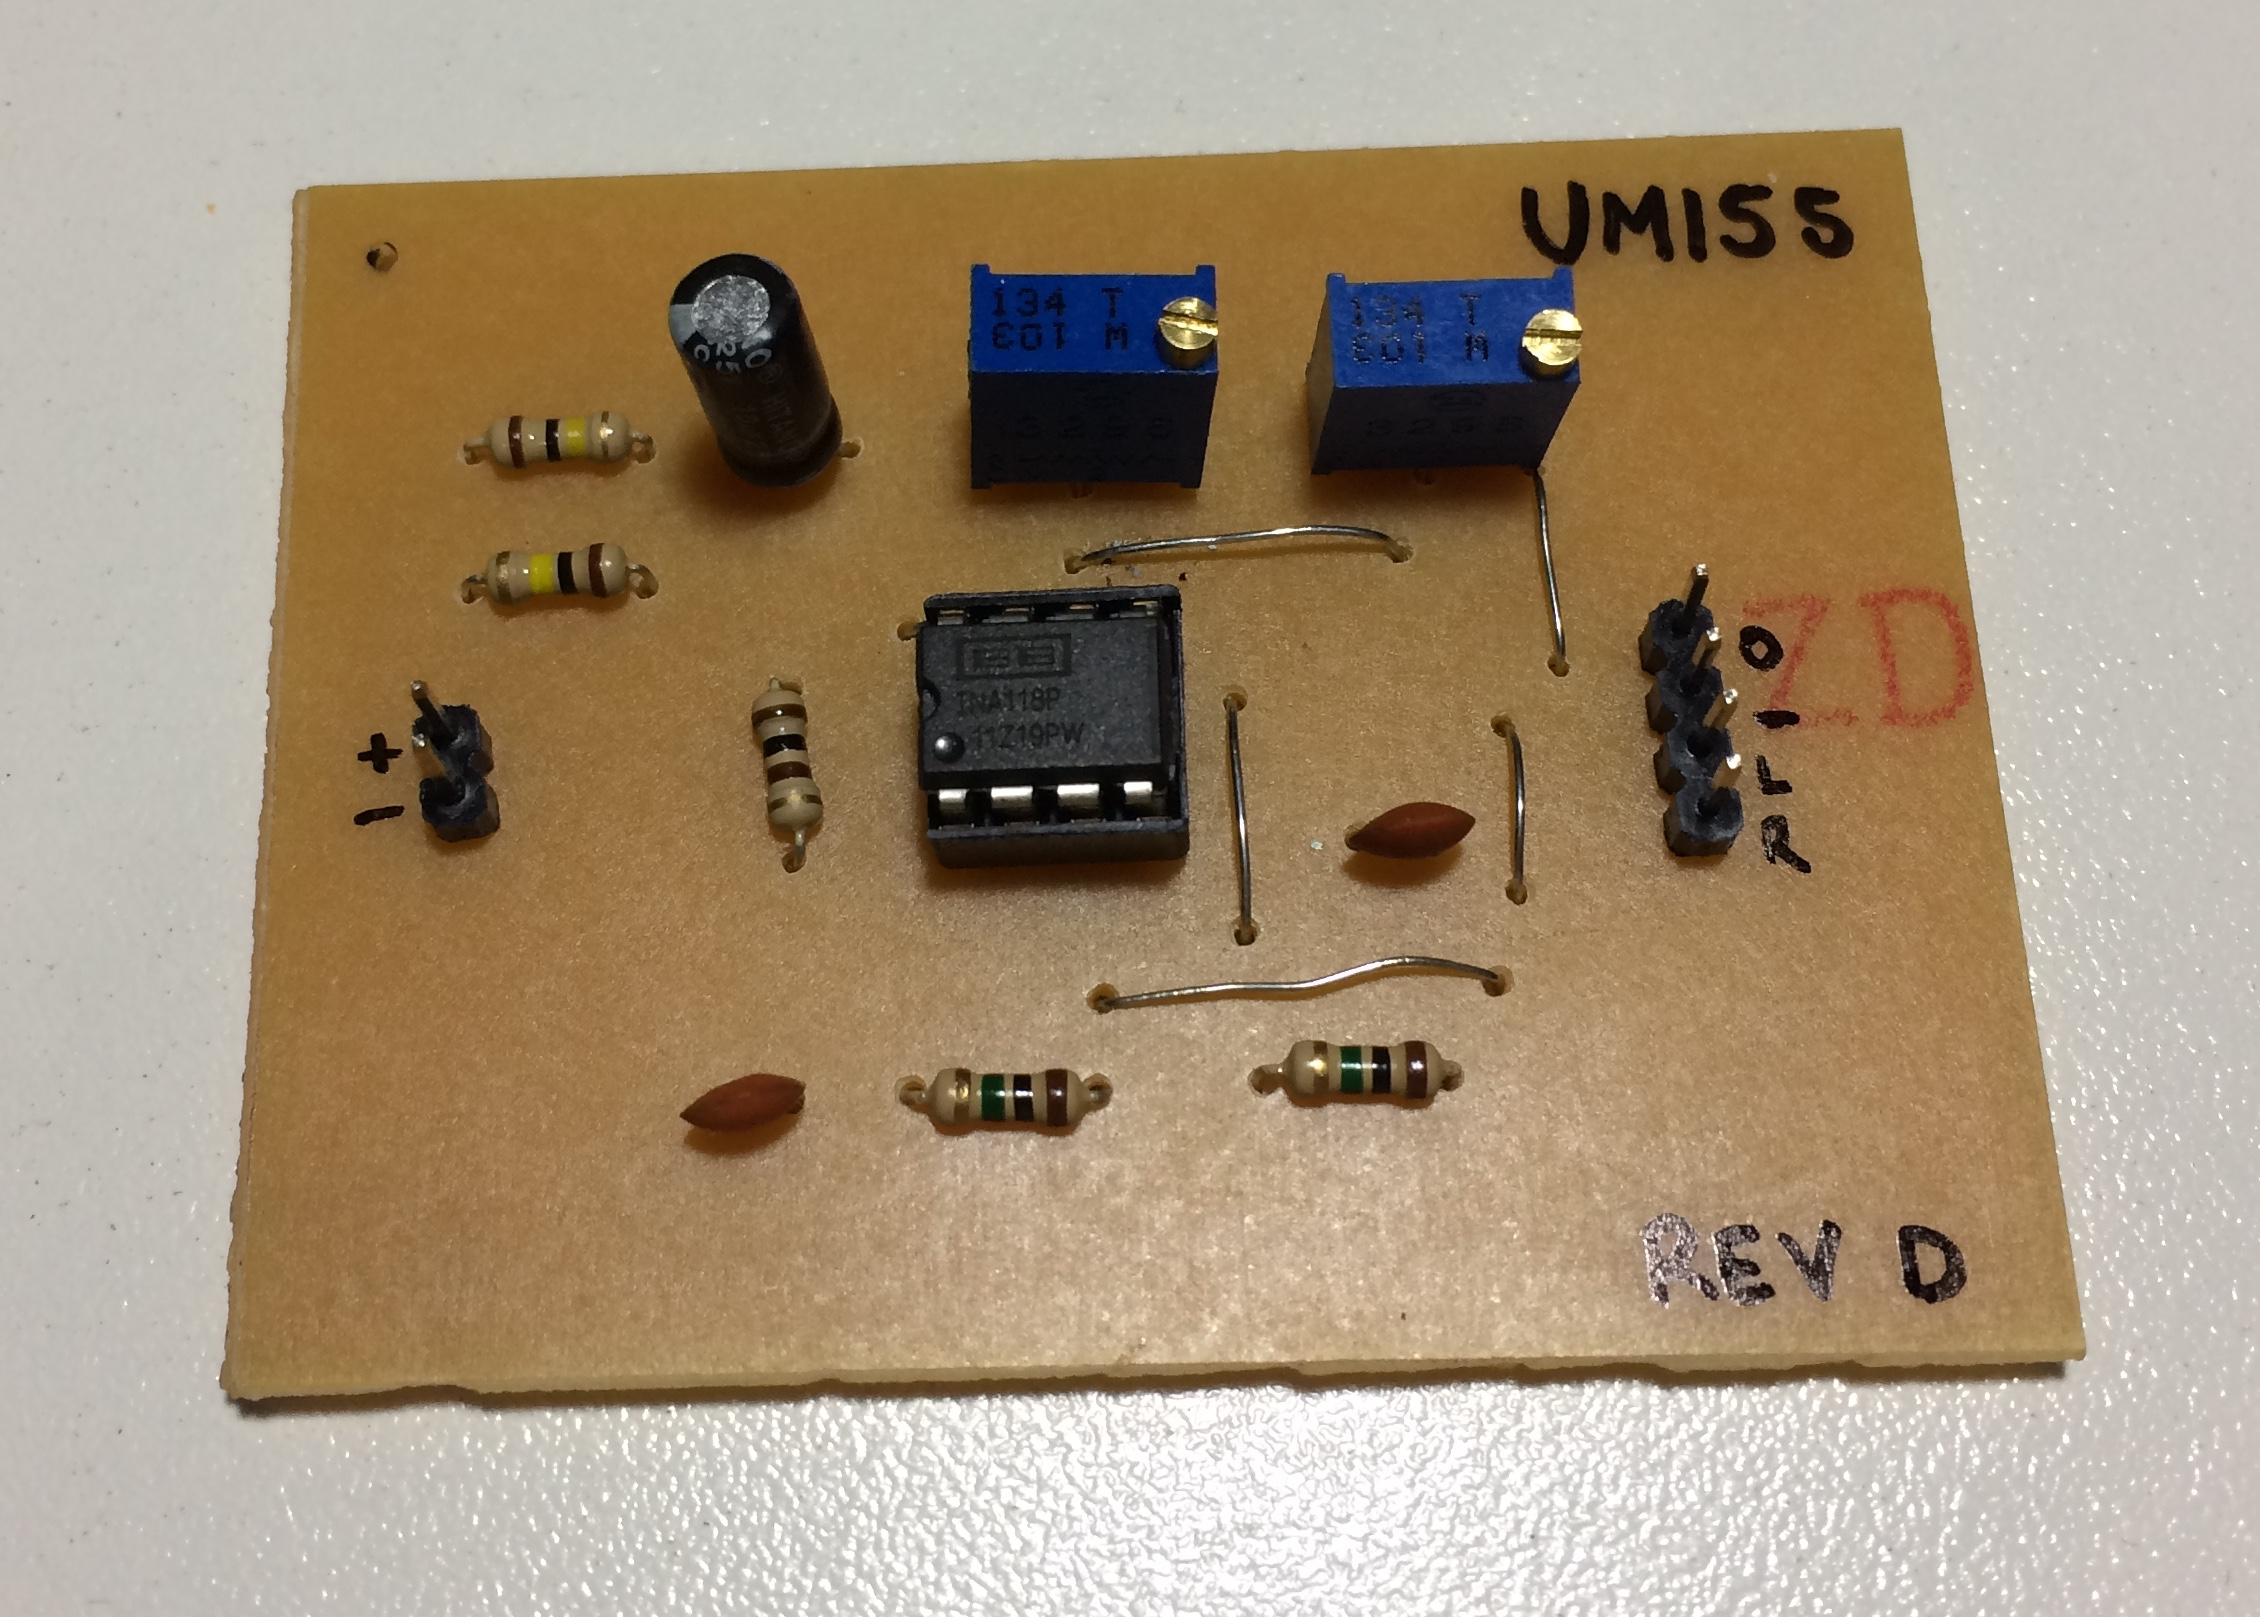
\includegraphics[scale=0.1]{figuras/ecg_circ.jpg}
    \end{center}
    \caption{Circuito condicionador e de aquisição de sinais de eletrocardiograma.}
    \label{fig:ecg_ele}
\end{figure}

O projeto de captura dos sinais de eletrocardiograma utilizando o amplificador INA128
é dado a partir do ganho necessário para a visualização e processamento do sinal, com isso,
o ganho do amplificador é dado pela equação:

\begin{equation}
  Av = 1 + \frac{50000}{R_{G}}
\end{equation}}

Sabe-se que a amplitude de sinais de ECG é baixa, na faixa de 0.1 $mV$ a 5 $mV$.
Com isso, foi implementado um resistor $R_{G} = 100 \omega$, resultando em um ganho
$Av = 501$. Dessa forma, o sinal terá uma amplitude de cerca de 2.5 $V$.

Após testes, os primeiro sinais obtidos foram satisfatórios para monitoramento de frequência
cardíaca. Dessa forma, após o condicionamento, os sinais são enviados para um microcontrolador Arduino,
que realiza a amostragem e envia os dados de forma Serial para o processador princial presente na
Raspberry Pi, onde os dados são capturados pela porta USB, e dispostos em um \textit{array}, alterado
a cada periodo de tempo. Para teste de visualização destes dados, os mesmo foram plotados no sistema
da Raspberry Pi utilizando a biblioteca \textit{matplotlib}\footnote{\url{https://matplotlib.org/}}.

Após a captura e condicionamento de todos os sinais analógicos, os mesmos são direcionados
para um módulo de conversão Analógico-Digital (A/D). O conversor selecionado foi o ADS1115 \footnote{\url{https://cdn-shop.adafruit.com/datasheets/ads1115.pdf}},
devido a sua alta resolução de 16 bits, capaz de converter valores analógicos em valores
digitais de 0 a 65535, e por sua taxa de amostragem de 800Hz, suficientes para a captura dos
sinais a serem monitorados para o projeto. O conversor é conectado com a Raspberry Pi via protocolo I2C,
possibilitando o uso de menos portas para o envio de até 4 sinais simultâneos.


\begin{figure}
    \begin{center}
        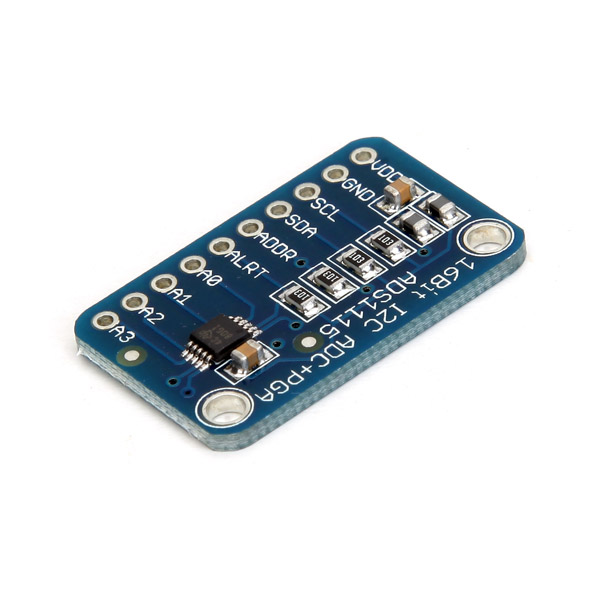
\includegraphics[scale=0.5]{figuras/ads.jpg}
    \end{center}
    \caption{Conversor A/D ADS1115.}
    \label{fig:ads}
\end{figure}

Uma vez com os sinais devidamente convertidos para digital, o sistema embarcado e de \textit{middleware}
é responsável por monitorar os sinais, realizando verificações de seus valores a partir de calibrações
realizadas para cada um dos módulos.
